\section{Auswertung}
\label{sec:Auswertung}

\subsection{Zeitabhängigkeit der Amplitude}

%Aufgabe a
Die Form der Einhüllenden ist, da $\mathit{U(t) \propto I(t)}$, nach Gleichung xy durch
\begin{align*}
A = A_\text{0} \mathrm{e}^{-2 \pi \mu t}
\end{align*}
gegeben.


Die aufgenommenen Wertepaare der Spannungsamplitude $U_\text{C}$ und der Zeit $t$
befinden sich in Tabelle 1. Mithilfe exponentieller Regression mittels Python erhält man
\begin{align*}
A_\text{0} &= (\num{31,32 +- 0,63})\,\mathrm{V} \\
\mu &= (\num{194.51 +- 13.15})\,\mathrm{\frac{1}{s}} .
\end{align*}

\begin{table}[H]
\centering
\caption{Messdaten zur Bestimmung des effektiven Dämpfungswiderstandes sowie der Abklingdauer.}
\label{tab:some_data}
\begin{tabular}{c c c c}
\toprule
$U_\text{C} \:/\: V$ & $t \:/\: 10^{-6}\si{\second}$ & $U_\text{C} \:/\: V$ & $t \:/\: 10^{-6}\si{\second}$\\
\midrule
20  & 32,2 & 286 & 21,2\\
58  & 29,8 & 322 & 20,6\\
96  & 27,6 & 362 & 20,4\\
134 & 25,8 & 398 & 19,8\\
172 & 24,6 & 436 & 19,4\\
210 & 23,4 & 474 & 18,8\\
248 & 22 \\
\bottomrule
\end{tabular}
\end{table}

Über Gleichung xy ergibt sich dann für den effektiven Dämpfungswiderstand
$R_\text{eff}$ und der Abklingdauer $T_\text{ex}$ 
\begin{align*}
R_\text{eff} &= (\num{41.0 +- 2.8})\,\si{\ohm}\\
T_\text{ex} &= (\num{820 +- 60})\,\mathrm{µs}.
\end{align*}
Die zugehörigen Fehler ergeben sich durch die Gauß'sche Fehlerfortpflanzung der Form
\begin{align*}
\sigma_{R_\text{eff}} &= \sqrt{ 16 L^{2} \pi^{2} \sigma_{\mu}^{2} + 16 \mu^{2} \pi^{2} \sigma_{L}^{2}} \\
\sigma_{T_\text{ex}} &= \sqrt{\frac{4 L^{2} \sigma_{R_\text{eff}}^{2}}{R_\text{eff}^{4}} + \frac{4 \sigma_{L}^{2}}{R_\text{eff}^{2}}}.
\end{align*}

\begin{figure}[H]
  \centering
  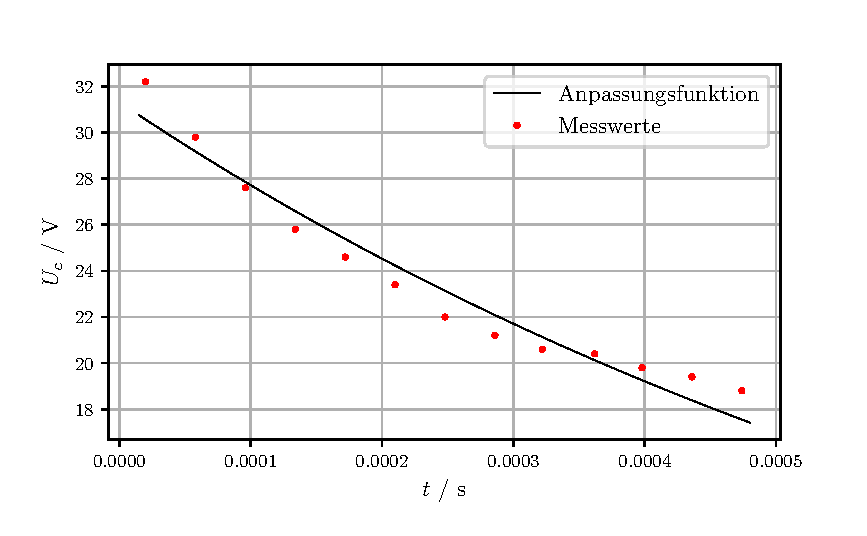
\includegraphics{plota.pdf}
  \caption{Abklingvorgang des gedämpften $\mathit{RLC}$-Schwingkreises und Ausgleichsfunktion.}
  \label{fig:Plot a}
\end{figure}

\subsection{Bestimmung des Dämpfungswiderstands }
%Aufgabe b
Der Dämpfungswiderstand, für den der aperiodische Grenzfall eintrifft, wird als 
\begin{align*}
R_\text{ap,ex} = \SI{3,05}{\kilo\ohm}
\end{align*}
gemessen.
Der theoretische Wert des Dämpfungswiderstandes wird mit Gleichung xy berechnet.
Der Fehler errechnet sich über die Gauß'sche Fehlerfortpflanzung:
\begin{align*}
\sigma_{R_\text{ap,th}} = \sqrt{\frac{\sigma_{L}^{2}\frac{L}{C}}{L^{2}} + \frac{\sigma_{C}^{2} \frac{L}{C}}{C^{2}}}
\end{align*}
Somit ergibt sich für den theoretischen Dämpfungswiderstand
\begin{align*}
R_\text{ap,th} = \SI{5.7 \pm 0.02}{\kilo\ohm}.
\end{align*}

%Aufgabe c
\subsection{Frequenzabhängigkeit der Kondensatorspannung}
Die zur Berechnung der Resonanzüberhöhung $q$ aufgenommenen Wertepaare, bestehend aus der Spannungsamplitude $U_c$ und der Frequenz $f$, befinden sich zusammen mit der
normierten Spannungsamplitude in Tabelle 2. Ferner sind sie normierten Kondensatorspannungen in Abbildung 2 gegen die Frequenz aufgetragen.
Die Resonanzüberhöhung 
\begin{align*}
q_\text{ex} &= \num{3.8}
\end{align*}
wird dem Graphen entnommen. Mit der Gleichung xy ergibt sich für den theoretischen Wert der Resonanzüberhöhung 
\begin{align*}
q_\text{th} &= \num{4.179 +-0.014},
\end{align*}
wobei der Fehler mit der Gauß'schen Fehlerfortpflanzung in der Form
\begin{align*}
\sigma_{q_\text{th}} = \sqrt{\frac{L \sigma_{C}^{2}}{4C^{3} R^{2}} + \frac{\sigma_{L}^{2}}{4C L R^{2}} + \frac{L \sigma_{R}^{2}}{C R^{4}}}
\end{align*}
ermittelt wird.

\begin{table}
\centering
\caption{Messdaten zur Bestimmung Resonanzüberhöhung $q_\text{ex}$.}
\label{tab:some_data}
\begin{tabular}{c c c c c c c c c}
\toprule
$\mathit{U_c \: / \: \mathrm{V}}$ & $\frac{U_c}{U_0}$ & $\mathit{f \: / \: \mathrm{KHz}}$ & $\mathit{U_c \: / \: \mathrm{V}}$ & $\frac{U_c}{U_0}$ & $\mathit{f \: / \: \mathrm{KHz}}$ & $\mathit{U_c \: / \: \mathrm{V}}$ & $\frac{U_c}{U_0}$ & $\mathit{f \: / \: \mathrm{KHz}}$ \\
\midrule
2  & 1     & 10,2 & 23 & 2,980  & 30,4 & 36 & 1,019  & 10,6 \\
4  & 1,019  & 10,4 & 24 & 3,333  & 34 & 38 & 0,846  &  8,8 \\
6  & 1,038  & 10,8 & 25 & 3,7    & 37 & 40 & 0,711  &  7,4 \\
8  & 1,056  & 11,2 & 26 & 3,78   & 37,8 & 42 & 0,596  &  6,2 \\
10 & 1,074  & 11,6 & 27 & 3,58   & 35,8 & 44 & 0,519  &  5,4 \\
12 & 1,169  & 12,4 & 28 & 3,18   & 31,8 & 46 & 0,452  &  4,8 \\
14 & 1,283  & 13,6 & 29 & 2,705  & 27,6 & 48 & 0,396  &  4,2 \\
16 & 1,433  & 15,2 & 30 & 2,313  & 23,6 & 50 & 0,358  &  3,8 \\
18 & 1,660  & 17,6 & 31 & 1,942  & 20,2 & 52 & 0,320  &  3,4 \\
20 & 2,019  & 21 & 32 & 1,673  & 17,4 & & & \\
22 & 2,423  & 25,2 & 34 & 1,288  & 13,4 & & & \\
\bottomrule
\end{tabular}
\end{table}

\begin{figure}[H]
  \centering
  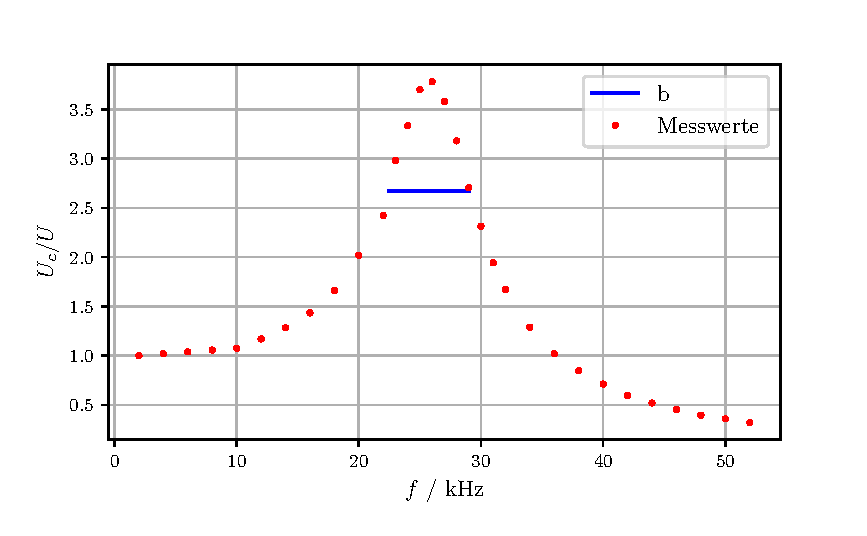
\includegraphics{plotc.pdf}
  \caption{Lineare Darstellung der normierten Kondensatorspannung $\frac{U_\text{C}}{U_\text{0}}$ in Abhängigkeit der Frequenz $f$.}
  \label{fig:Plot c}
\end{figure}

Der experimentelle Wert der Halbwertsbreite $b_\text{ex}$ wird aus der Abbildung als
\begin{align*}
b_\text{ex} = 6\,500\frac{1}{s}
\end{align*}
abgelesen. Mit Gleichung xy wird die theoretiche Halbwertsbreite 
\begin{align*}
b_\text{th} &= (6\,470 \pm 40)\frac{1}{s}
\end{align*}
bestimmt. Der zugehörige Fehler wird über die Gauß'sche Fehlerfortpflanzung 
\begin{align*}
\sigma_{b_\text{th}} = \sqrt{\frac{\sigma_{R}^{2}}{2 \pi L^{2}} + \frac{R^{2} \sigma_{L}^{2}}{2 \pi L^{4}}}
\end{align*}
ermittelt.
%Aufgabe d
\subsection{ Frequenzabhängigkeit der Phasenverschiebung}
In Abbildung 3 erkennt man für die Phasenverschiebung benötigten Parameter a und b. Die Phasenverschiebung lässt sich nun wie folgt errechnen:
\begin{align*}
\phi = \frac{a}{b} \cdot 2\pi
\end{align*}
Leider können wir an dieser Stelle durch die Annahme, dass der Parameter a konstant Null ist, keine brauchbaren Ergebnissen liefern. In Tabelle 3
befinden sich die dazugehörigen Messwerte.

\begin{table}
\centering
\caption{Messdaten zur Bestimmung der frequenzabhängigen Phasenverschiebung.}
\label{tab:some_data}
\begin{tabular}{c c}
\toprule
$\mathit{f \: / \: \mathrm{KHz}}$ & $\mathit{T \: \text{in $10^{-6}$} \: \mathrm{s}}$ \\
\midrule
15 & 67 \\
20 & 50 \\
25 & 40 \\
30 & 33.6 \\
31 & 32.4 \\
32 & 31.2 \\
33 & 30.4 \\
34 & 29.6 \\
35 & 28.8 \\
36 & 27.6 \\
37 & 27.2 \\
38 & 26.4 \\
39 & 26 \\
40 & 25.2 \\
45 & 22.4 \\
50 & 20.4 \\
55 & 18.4 \\
60 & 16.8 \\
\bottomrule
\end{tabular}
\end{table}
